
\par\noindent\textit{引理~\ref{lem:7-2-291} 的证明.}\quad
(7.2.292.1) 的证明与引理 7.2.136 相同。

先证 (7.2.292.2)。设 $\mathfrak P$ 是满足
定义~\ref{def:7-2-288} 的 $m$ 维奇异单形。
不妨设它不包含于
$[0,1]^2\times L'_1$ 的边界。
设 $\Delta_b^{m-2}$ 是包含于
$f^{-1}(\{r_0\}\times\{s_0\}\times L'_1)$
的一个 $m-2$ 维面。
\translatornote{原书此处把角点坐标写作
$(s_0,r_0)$；本小节一直按 $(r,s)$ 排列，
故按定义 7.2.288 改作 $(r_0,s_0)$。}
要证明 $\Delta_b^{m-2}$ 在
\begin{equation}
\bigl(\operatorname{Eval}_{r=r_0}\circ
\operatorname{Eval}_{s=s_0}
-\operatorname{Eval}_{s=s_0}\circ
\operatorname{Eval}_{r=r_0}\bigr)(\mathfrak P)
\tag{7.2.293}\label{eq:7-2-293}
\end{equation}
中的系数为零。
由于 $\mathfrak P$ 与角点相交，
它满足 (7.2.289.3) 的 (i) 或 (ii)。
若满足 (i)，(7.2.293) 的两项都为零。
下面设满足 (ii)。于是
\[
\begin{aligned}
\dim\bigl(f^{-1}((0,1)_r\times\{s_0\}\times L'_1)
\cap|\mathfrak P|\bigr)
&=m-1,\\
\dim\bigl(f^{-1}(\{r_0\}\times(0,1)_s\times L'_1)
\cap|\mathfrak P|\bigr)
&=m-1.
\end{aligned}
\]
也就是说，在 $s=s_0$、$r=r_0$ 的逆像中
分别有余维一的面
$\Delta_c^{m-1}$、$\Delta_{c'}^{m-1}$，
其边界都包含 $\Delta_b^{m-2}$。
因而
\[
\begin{aligned}
(\operatorname{Eval}_{r=r_0}\circ
\operatorname{Eval}_{s=s_0})(\mathfrak P)
&=(-1)^{s_0+c}
\operatorname{Eval}_{r=r_0}
(\Delta_c^{m-1},f|_{\Delta_c^{m-1}})\\
&=(-1)^{s_0+c+r_0+c'-\epsilon+1}
(\Delta_b^{m-2},f|_{\Delta_b^{m-2}}),\\
(\operatorname{Eval}_{s=s_0}\circ
\operatorname{Eval}_{r=r_0})(\mathfrak P)
&=(-1)^{r_0+c'+1}
\operatorname{Eval}_{s=s_0}
(\Delta_{c'}^{m-1},f|_{\Delta_{c'}^{m-1}})\\
&=(-1)^{r_0+c'+1+s_0+c-(1-\epsilon)+1}
(\Delta_b^{m-2},f|_{\Delta_b^{m-2}}),
\end{aligned}
\]
其中当 $c'<c$ 时 $\epsilon=0$，
当 $c<c'$ 时 $\epsilon=1$。
两式的符号相同，故 (7.2.292.2) 得证。

再证 (7.2.292.3)。由于
$\operatorname{Eval}\circ\operatorname{Incl}$
在同调上是恒等，只须证明
$\operatorname{Eval}$ 在同调上单射。
设 $\mathfrak C=\sum_{i\in I}\mathfrak P_i$
是 $S([0,1]^2\times L'_1)$ 中的一个
$m$ 维循环，且\translatornote{原书在此把带方括号的同调类
写成属于链复形 $S([0,1]_r\times\{0\}\times L'_1)$；
下页选取边界填充链，表明此处所需的是同调类为零。}
\[
[\operatorname{Eval}_{s=0}(\mathfrak C)]=0
\quad\text{于相应同调群中}.
\]
由 (7.2.292.2)、(7.2.175.4) 还得
\[
[\operatorname{Eval}_{s=1}(\mathfrak C)]=0,
\qquad
[\operatorname{Eval}_{r=0}(\mathfrak C)]=0,
\qquad
[\operatorname{Eval}_{r=1}(\mathfrak C)]=0.
\]
取 $m$ 维奇异链\translatornote{原书把所有
$\mathfrak D_{s=s_0}$ 都放在 $s=0$ 端面；
当 $s_0=1$ 时，它应位于 $s=s_0$ 端面，
方能以该端评价链为边界。}
\[
\begin{aligned}
\mathfrak D_{s=s_0}&\in
S([0,1]_r\times\{s_0\}\times L'_1),\\
\mathfrak D_{r=r_0}&\in
S(\{r_0\}\times[0,1]_s\times L'_1),
\end{aligned}
\]
满足
\[
\operatorname{Eval}_{s=s_0}(\mathfrak C)
=\partial\mathfrak D_{s=s_0},
\qquad
\operatorname{Eval}_{r=r_0}(\mathfrak C)
=\partial\mathfrak D_{r=r_0}.
\]
如第 7.2.10 小节那样，
可取 $\mathfrak C$ 的代表
\[
\mathfrak C'
=\mathfrak C-
\sum_{s_0=0,1}\mathfrak D_{s=s_0}
-\sum_{r_0=0,1}\mathfrak D_{r=r_0}
\in S_+([0,1]^2\times L'_1).
\]
于是 $\partial\mathfrak C'$ 是由像包含于
$\{0,1\}\times\{0,1\}\times L'_1$
的奇异单形之和。
设 $\mathfrak X_{r_0,s_0}$ 是
$\partial\mathfrak C'$ 中所有与
$\{r_0\}\times\{s_0\}\times L'_1$
相交的奇异单形之和。则
\[
(\operatorname{Incl}_s)_{1,\beta_0}
(\mathfrak X_{r_0,s_0})
\in S(\{r_0\}\times[0,1]_s\times L'_1)
\subset S_+([0,1]^2\times L'_1).
\]
记
$(\operatorname{Incl}_s)'_{1,\beta_0}
(\mathfrak X_{r_0,s_0})$
为上述 $\operatorname{Incl}_s$ 奇异链中
与 $\mathfrak X_{r_0,s_0}$ 相交的那些奇异链之和。
置
\[
\mathfrak C''=\mathfrak C'
-\sum_{r_0,s_0}
(\operatorname{Incl}_s)'_{1,\beta_0}
(\mathfrak X_{r_0,s_0}).
\]
则 $\partial\mathfrak C''$ 中各奇异单形的像
均包含于
$[0,1]_r\times([0,1]_s\setminus
\partial[0,1]_s)\times L'_1$。

设 $\{\mathfrak P_a\}_{a\in A}$ 是
$\mathfrak C''$ 中所有与
$\{(0,0)\}\times L'_1$ 相交的单形，
$c_a$ 为其系数；记
$\mathfrak P_a=(|\mathfrak P_a|,f_a)$。
存在 $\epsilon>0$，使对所有 $a$ 都有
\[
f_a(|\mathfrak P_a|)
\subset[0,1/3-\epsilon)^2\times L'_1.
\]
记
$f_a=(f_{a,r},f_{a,s},f_{a,L'_1})$，
定义
$\widehat f_a\colon
|\mathfrak P_a|\times[0,1]
\to[0,1]^2\times L'_1$ 为\translatornote{原书式 (7.2.294) 的第一、三分量
写 $f_{i,r}$、$f_{i,L'_1}$；本段只定义了
$f_a$，故依紧前的分量分解改为下标 $a$。}
\begin{equation}
\widehat f_a(x,t)
=\bigl(f_{a,r}(x),
\epsilon t/2+f_{a,s}(x),
f_{a,L'_1}(x)\bigr).
\tag{7.2.294}\label{eq:7-2-294}
\end{equation}
\begin{statement}{子引理}{7.2.295}\label{sublem:7-2-295}
可以对 $|\mathfrak P_a|\times[0,1]$
取棱柱剖分\liftIndex{I279}，
使 $\widehat f_a$ 在每个最高维单形上的限制都适配。
特别地，这种剖分给出
$S_+([0,1]^2\times L'_1)$ 中的一个元素。
\end{statement}

暂设子引理~\ref{sublem:7-2-295} 成立，
先完成 (7.2.292.3) 的证明。
令 $\Psi_{0,0}(\mathfrak P_a)$ 表示由子引理得到的
$S_+([0,1]^2\times L'_1)$ 中的奇异链。
容易证明
\[
\partial\Psi_{0,0}(\mathfrak P_a)
-\Psi_{0,0}(\partial\mathfrak P_a)
-\mathfrak P_a
\]
不与 $\{(0,0)\}\times L'_1$ 相交。
定义
\[
\mathfrak C'''=\mathfrak C''-
\sum_{a\in A}c_a\partial\Psi_{0,0}(\mathfrak P_a).
\]
于是 $\mathfrak C'''$ 不与
$\{(0,0)\}\times L'_1$ 相交。
事实上，$\sum_{a\in A}c_a\partial\mathfrak P_a$
也不与这个角点相交，因为
$\partial\mathfrak C''$ 不与它相交。

在另外三个角点
$\{(1,0)\}\times L'_1$、
$\{(0,1)\}\times L'_1$、
$\{(1,1)\}\times L'_1$
重复此构造。于是可以且将假定循环
$\mathfrak C$ 不与 $[0,1]^2\times L'_1$
的任何角点相交。

设 $\{\mathfrak P_a\}_{a\in A}$ 是
$\mathfrak C$ 中所有与
$[0,1]_r\times\{0\}\times L'_1$ 相交的单形，
记这些单形构成的子链为\translatornote{原书此处把所选的“与 $s=0$ 端面相交的
单形之和”直接写成整个 $\mathfrak C$；
其余不碰该端面的单形仍可存在，
故这里把求和限定为相应子链，后续仍对整个循环作修正。}
\[
\mathfrak C_{s=0}
=\sum_{a\in A}c_a\mathfrak P_a.
\]
令 $\mathfrak P_a=(|\mathfrak P_a|,f_a)$，
按 (7.2.294) 定义 $\widehat f_a$。
由于 $\mathfrak P_a$ 不与角点相交，
棱柱剖分把
$(|\mathfrak P_a|\times[0,1],\widehat f_a)$
分解成适配单形。
将所得链记作 $\Psi_0(\mathfrak P_a)$。
于是
\[
\mathfrak C-
\sum_{a\in A}c_a\partial\Psi_0(\mathfrak P_a)
\]
不与 $[0,1]_r\times\{0\}\times L'_1$ 相交。
在 $s=1$ 端面重复此构造，
便可且将假定 $\mathfrak C$ 不与
$[0,1]_r\times\partial[0,1]_s\times L'_1$
相交。

最后重复引理 7.2.136 的证明：把
$[0,1]^2\times L'_1$ 看成
$[0,1]_r\times([0,1]_s\times L'_1)$，
在该引理的证明中以这里的 $[0,1]_r$
充当区间参数。由此 $\mathfrak C$ 是边界，
(7.2.292.3) 得证。

\par\noindent\textit{子引理~\ref{sublem:7-2-295} 的证明.}\quad
只需验证 (7.2.289.3)，
其余条件容易检查。
设 $f_a\colon|\mathfrak P_a|\to
[0,1/3-\epsilon)^2\times L'_1$ 如上。
若 $f_a(|\mathfrak P_a|)$ 包含于
$\partial([0,1/3-\epsilon)^2\times L'_1)$，
则 (7.2.289.3) 易证。
故可设 $f_a(|\mathfrak P_a|)$ 同时与
$\{0\}\times(0,1/3-\epsilon)_s\times L'_1$
及 $(0,1/3-\epsilon)_r\times\{0\}\times L'_1$
相交。

首先，$\mathfrak P_a$ 不可能有顶点 $v$ 满足
$f_a(v)\in(0,1/3-\epsilon)^2\times L'_1$。
否则可把它与满足
$f_a(v_0)\in\{(0,0)\}\times L'_1$
的顶点 $v_0$ 相连，所得一维面便违反
(7.2.289.3)。

考虑三角形
\[
\Delta^2=\{(\sigma,\rho)
\mid 0\le\sigma,\rho,\ \sigma+\rho\le1\},
\]
定义仿射映射
$\psi\colon|\mathfrak P_a|\to\Delta^2$，
使其在顶点上满足：
\begin{enumerate}[label=\textup{(\arabic*)},leftmargin=3.5em]
\item 若 $v\in|\mathfrak P_a|$ 位于
$\{(0,0)\}\times L'_1$，则 $\psi(v)=(0,0)$；
\item 若 $v\in|\mathfrak P_a|$ 位于
$\{0\}\times(0,1/3)_s\times L'_1$，
则 $\psi(v)=(0,1)$；
\item 若 $v\in|\mathfrak P_a|$ 位于
$(0,1/3)_r\times\{0\}\times L'_1$，
则 $\psi(v)=(1,0)$。
\end{enumerate}
见图~\ref{fig:7-2-15}。

先考虑 $\dim\mathfrak P_a=2$。
此时可将 $|\mathfrak P_a|$ 与 $\Delta^2$ 识别。
可以选取棱柱剖分，使顶点
$(0,0,0)$ 不与 $(1,0,1)$ 相连。
注意，$\widehat f_a^{-1}((0,1/3)^2\times L'_1)$
只含一个顶点 $(1,0,1)$，而
$\widehat f_a^{-1}(\{(0,0)\}\times L'_1)$
只含一个顶点 $(0,0,0)$。
此外，棱柱剖分不改变顶点集，
故此时容易验证 (7.2.289.3)。

一般情形下，考虑仿射映射
\[
\psi\times\operatorname{id}\colon
|\mathfrak P_a|\times[0,1]
\longrightarrow\Delta^2\times[0,1].
\]
把上述 $\Delta^2\times[0,1]$ 的单纯剖分
拉回到 $|\mathfrak P_a|\times[0,1]$，
得到其上的一个剖分
（此时未必已是单纯剖分）。
可选棱柱剖分，使它细分这个拉回剖分。
对该剖分容易验证 (7.2.289.3)。
子引理~\ref{sublem:7-2-295} 得证。$\square$

\par\medskip\noindent\begin{minipage}{\textwidth}
\centering
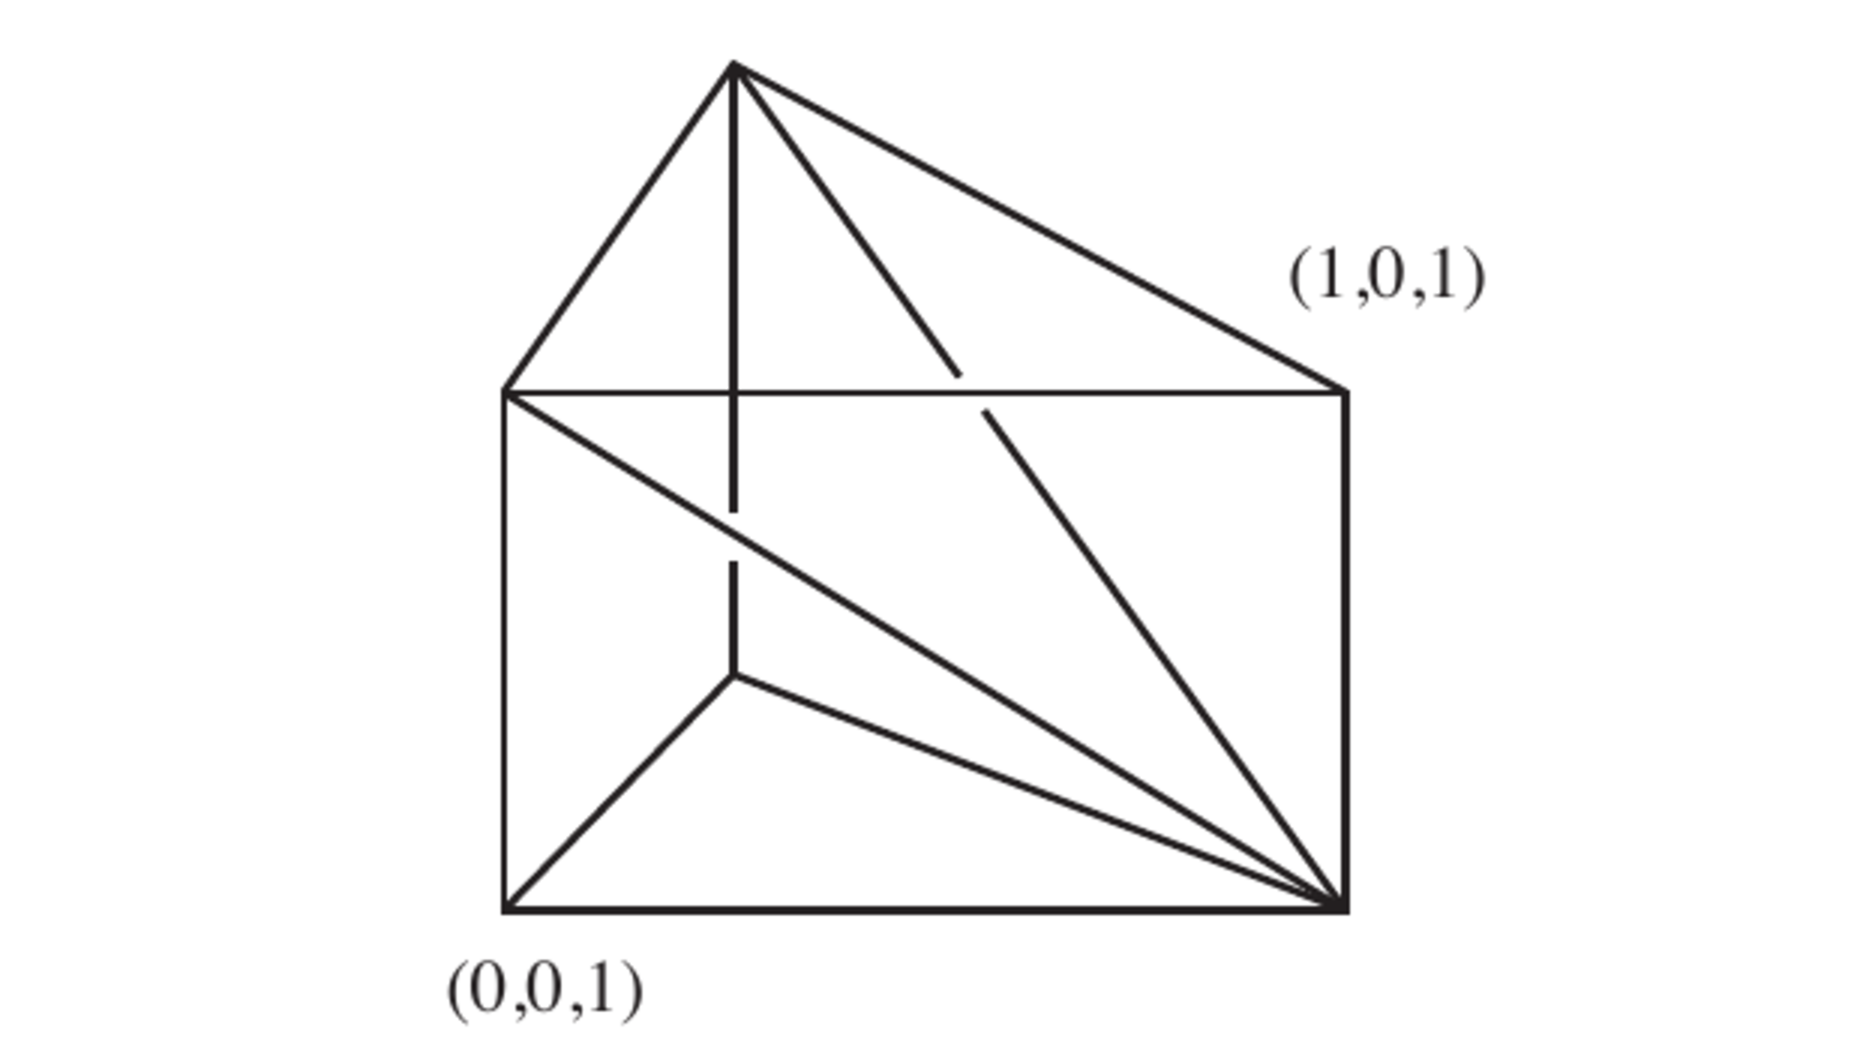
\includegraphics[width=.50\textwidth]{chapters/ch07-transversality/figures/phys-555-figure-7-2-15-math3-crop.png}
\par{\renewcommand{\thefigure}{7.2.15}\refstepcounter{figure}
\normalfont\bfseries 图~\thefigure\label{fig:7-2-15}}
\end{minipage}\par\medskip
